\subsection{Study Design}

To investigate the usability of the developed feedback schemes in combination with control an experiment was conducted which evaluated the usefulness of the feedback schemes when eliminating visual dependency. For this purpose 14 able-bodied subjects (12 male and 2 female - 13 right-handed and 1 left-handed with a mean age of $26.1 \pm 2.4$ ) were recruited. Included subjects signed an informed consent form and meet inclusion criteria stated in the experimental protocol, which was ethically approved by the ethical committee of Region Nordjylland, Denmark (approval number N-20150075). Each subject was introduced, trained and finally evaluated in understanding both the spatially based scheme and the amplitude based scheme. However, the order of which feedback scheme the subject would be trained/tested in was randomized. Figure \ref{fig:pa:std_pap} illustrates the chronological flow of stages in the experiment, where the first block focused on developing a subject specific prosthetic control system and the second block focused on training and evaluating the use of the sensory feedback schemes. 
During the first block, EMG data was initially acquired and used to train a control system, which was used for a simulate prosthetic control. Subsequently, was a stage where the subject was made familiar with the control system. Finally, the achieved prosthetic control was evaluated through a target reaching test. Afterwards, a series of subjects sensory thresholds were determined for use of conveying electrotactile feedback. The subject then began the stages of familiarizing and training with a feedback scheme followed by re-familiarization of control in combination with feedback. Finally, a evaluation test of using the sensory feedback in combination for control was made. The entire sensory feedback block was then repeated using the remaining feedback scheme. 

\begin{figure}[H]                 
	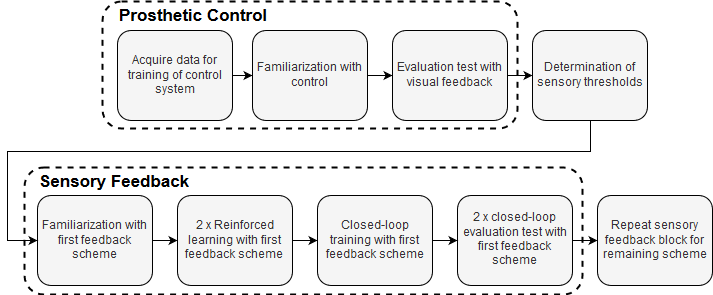
\includegraphics[width=1\textwidth]{figures/std_paper}
	\caption{Pipeline showing the stages of the experiment. The stages in the first block focused on developing and evaluating a subject specific simulated prosthetic control system. Then electrotactile sensory thresholds were determined. The second block focused on training the understanding of the feedback schemes and evaluating their use in combination with prosthetic control.}
	\label{fig:pa:std_pap} 
\end{figure}


